% -*- coding: utf-8 -*-
%\documentclass[output=paper]{LSP/langsci} 
\documentclass[output=paper
,newtxmath
,modfonts
,nonflat]{langsci/langscibook} 
% \bibliography{localbibliography} 
% \usepackage{pifont}
\usepackage{savesym}

\savesymbol{downingtriple}
\savesymbol{downingdouble}
\savesymbol{downingquad}
\savesymbol{downingquint}
\savesymbol{suph}
\savesymbol{supj}
\savesymbol{supw}
\savesymbol{sups}
\savesymbol{ts}
\savesymbol{tS}
\savesymbol{devi}
\savesymbol{devu}
\savesymbol{devy}
\savesymbol{deva}
\savesymbol{N}
\savesymbol{Z}
\savesymbol{circled}
\savesymbol{sem}
\savesymbol{row}
\savesymbol{tipa}
\savesymbol{tableauxcounter}
\savesymbol{tabhead}
\savesymbol{inp}
\savesymbol{inpno}
\savesymbol{g}
\savesymbol{hanl}
\savesymbol{hanr}
\savesymbol{kuku}
\savesymbol{ip}
\savesymbol{lipm}
\savesymbol{ripm}
\savesymbol{lipn}
\savesymbol{ripn} 
% \usepackage{amsmath} 
% \usepackage{multicol}
\usepackage{qtree} 
\usepackage{tikz-qtree,tikz-qtree-compat}
% \usepackage{tikz}
\usepackage{upgreek}


%%%%%%%%%%%%%%%%%%%%%%%%%%%%%%%%%%%%%%%%%%%%%%%%%%%%
%%%                                              %%%
%%%           Examples                           %%%
%%%                                              %%%
%%%%%%%%%%%%%%%%%%%%%%%%%%%%%%%%%%%%%%%%%%%%%%%%%%%%
% remove the percentage signs in the following lines
% if your book makes use of linguistic examples
\usepackage{tipa}  
\usepackage{pstricks,pst-xkey,pst-asr}

%for sande et al
\usepackage{pst-jtree}
\usepackage{pst-node}
%\usepackage{savesym}


% \usepackage{subcaption}
\usepackage{multirow}  
\usepackage{./langsci/styles/langsci-optional} 
\usepackage{./langsci/styles/langsci-lgr} 
\usepackage{./langsci/styles/langsci-glyphs} 
\usepackage[normalem]{ulem}
%% if you want the source line of examples to be in italics, uncomment the following line
% \def\exfont{\it}
\usetikzlibrary{arrows.meta,topaths,trees}
\usepackage[linguistics]{forest}
\forestset{
	fairly nice empty nodes/.style={
		delay={where content={}{shape=coordinate,for parent={
					for children={anchor=north}}}{}}
}}
\usepackage{soul}
\usepackage{arydshln}
% \usepackage{subfloat}
\usepackage{langsci/styles/langsci-gb4e} 
   
% \usepackage{linguex}
\usepackage{vowel}

\usepackage{pifont}% http://ctan.org/pkg/pifont
\newcommand{\cmark}{\ding{51}}%
\newcommand{\xmark}{\ding{55}}%
 
 
 %Lamont
 \makeatletter
\g@addto@macro\@floatboxreset\centering
\makeatother

\usepackage{newfloat} 
\DeclareFloatingEnvironment[fileext=tbx,name=Tableau]{tableau}
% %% hyphenation points for line breaks
%% Normally, automatic hyphenation in LaTeX is very good
%% If a word is mis-hyphenated, add it to this file
%%
%% add information to TeX file before \begin{document} with:
%% %% hyphenation points for line breaks
%% Normally, automatic hyphenation in LaTeX is very good
%% If a word is mis-hyphenated, add it to this file
%%
%% add information to TeX file before \begin{document} with:
%% %% hyphenation points for line breaks
%% Normally, automatic hyphenation in LaTeX is very good
%% If a word is mis-hyphenated, add it to this file
%%
%% add information to TeX file before \begin{document} with:
%% \include{localhyphenation}
\hyphenation{
affri-ca-te
affri-ca-tes
com-ple-ments
par-a-digm
Sha-ron
Kings-ton
phe-nom-e-non
Daul-ton
Abu-ba-ka-ri
Ngo-nya-ni
Clem-ents 
King-ston
Tru-cken-brodt
Tab-leau
cophono-logies
mark-edness
Ti-gri-nya
a-mong
Car-stens
Lu-bu-ku-su
}
\hyphenation{
affri-ca-te
affri-ca-tes
com-ple-ments
par-a-digm
Sha-ron
Kings-ton
phe-nom-e-non
Daul-ton
Abu-ba-ka-ri
Ngo-nya-ni
Clem-ents 
King-ston
Tru-cken-brodt
Tab-leau
cophono-logies
mark-edness
Ti-gri-nya
a-mong
Car-stens
Lu-bu-ku-su
}
\hyphenation{
affri-ca-te
affri-ca-tes
com-ple-ments
par-a-digm
Sha-ron
Kings-ton
phe-nom-e-non
Daul-ton
Abu-ba-ka-ri
Ngo-nya-ni
Clem-ents 
King-ston
Tru-cken-brodt
Tab-leau
cophono-logies
mark-edness
Ti-gri-nya
a-mong
Car-stens
Lu-bu-ku-su
}
% %add all your local new commands to this file
\newcommand{\downingquad}[4]{\parbox{2.5cm}{#1}\parbox{3.5cm}{#2}\parbox{2.5cm}{#3}\parbox{3.5cm}{#4}}
\newcommand{\downingtriple}[3]{\parbox{4.5cm}{#1}\parbox{3cm}{#2}\parbox{3cm}{#3}}
\newcommand{\downingdouble}[2]{\parbox{4.5cm}{#1}\parbox{6cm}{#2}}
\newcommand{\downingquint}[5]{\parbox{1.75cm}{#1}\parbox{2.25cm}{#2}\parbox{2cm}{#3}\parbox{3cm}{#4}\parbox{2cm}{#5}}
\newcolumntype{Y}{>{\centering\arraybackslash}X}
\newcolumntype{T}{>{\centering\arraybackslash}m{2cm}}

%commands for Kusmer paper below
\newcommand{\ip}{$\upiota$}
\newcommand{\lipm}{(\_{\ip-Max}}
\newcommand{\ripm}{)\_{\ip-Max}}
\newcommand{\lipn}{(\_{\ip}}
\newcommand{\ripn}{)\_{\ip}}
\renewcommand{\_}[1]{\textsubscript{#1}}


%commands for Pillion paper below
\newcommand{\suph}{\textipa{\super h}}
\newcommand{\supj}{\textipa{\super j}}
\newcommand{\supw}{\textipa{\super w}}
\newcommand{\ts}{\textipa{\t{ts}}}
\newcommand{\tS}{\textipa{\t{tS}}}
\newcommand{\devi}{\textipa{\r*i}}
\newcommand{\devu}{\textipa{\r*u}}
\newcommand{\devy}{\textipa{\r*y}}
\newcommand{\deva}{\textipa{\r*a}}
\renewcommand{\N}{\textipa{N}}
\newcommand{\Z}{\textipa{Z}}
% 

%commands for Diercks paper below
\newcommand{\circled}[1]{\begin{tikzpicture}[baseline=(word.base)]
\node[draw, rounded corners, text height=8pt, text depth=2pt, inner sep=2pt, outer sep=0pt, use as bounding box] (word) {#1};
\end{tikzpicture}
}

%commands for Pesetsky paper below
% \newcommand{\sem}[2][]{\mbox{$[\![ $\textbf{#2}$ ]\!]^{#1}$}}
\newcommand{\sem}[2][]{\mbox{$[[ $\textbf{#2}$ ]]^{#1}$}}

% \newcommand{\ripn}{{\color{red}ripn}}%this is used but never defined. Please update the definition



%commands for Lamont paper below
\newcommand{\row}[4]{
	#1. & 
    /{#2}/ & 
    [{#3}] & 
    `#4' \\ 
}
%\newcounter{tableauxcounter}
\newcommand{\tabhead}[2]{
%     \captionsetup{labelformat=empty}
%     \stepcounter{tableauxcounter}
%     \addtocounter{table}{-1}
% 	\centering
% 	\caption{Tableau \thetableauxcounter: #1}
	\caption{#1}
	\label{#2}
}
\newcommand{\candref}[2]{{(\ref{#1}#2)}}
\newcommand{\tableauref}[1]{{Tableau~\ref{#1}}}
% tableaux
\newcommand{\inp}[1]{\multicolumn{2}{|l||}{{#1}}}
\newcommand{\inpno}[1]{\multicolumn{2}{|l||}{#1}}
\newcommand{\g}{\cellcolor{lightgray}}
\newcommand{\hanl}{\HandLeft}
\newcommand{\hanr}{\HandRight}
\newcommand{\kuku}{Kuk\'{u}}

% \newcommand{\nocaption}[1]{{\color{red} Please provide a caption}}

% \providecommand{\biberror}[1]{{\color{red}#1}}

\definecolor{RED}{cmyk}{0.05,1,0.8,0}


\newfontfamily\amharicfont[Script = Ethiopic, Scale = 1.0]{AbyssinicaSIL}
\newcommand{\amh}[1]{{\amharicfont #1}}

% 
% %Gjersoe
\usepackage{textgreek}
% 
\newcommand{\viol}{\fontfamily{MinionPro-OsF}\selectfont\rotatebox{60}{$\star$}}
\newcommand{\myscalex}{0.45}
\newcommand{\myscaley}{0.65}
%\newcommand{\red}[1]{\textcolor{red}{#1}}
%\newcommand{\blue}[1]{\textcolor{blue}{#1}}
\newcommand{\epen}[1]{\colorbox{jgray}{#1}}
\newcommand{\hand}{{\normalsize \ding{43}}}
\definecolor{jgray}{gray}{0.8} 
\usetikzlibrary{positioning}
\usetikzlibrary{matrix}
\newcommand{\mora}{\textmu\xspace}
\newcommand{\si}{\textsigma\xspace}
\newcommand{\ft}{\textPhi\xspace}
\newcommand{\tone}{\texttau\xspace}
\newcommand{\word}{\textomega\xspace}
% \newcommand{\ts}{\texttslig}
\newcommand{\fns}{\footnotesize}
\newcommand{\ns}{\normalsize}
\newcommand{\vs}{\vspace{1em}}
\newcommand{\bs}{\textbackslash}   % backslash
\newcommand{\cmd}[1]{{\bf \color{red}#1}}   % highlights command
\newcommand{\scell}[2][l]{\begin{tabular}[#1]{@{}c@{}}#2\end{tabular}}
% \interfootnotelinepenalty=10000

% --- Snider Representations --- %

\newcommand{\RepLevelHh}{
\begin{minipage}{0.10\textwidth}
\begin{tikzpicture}[xscale=\myscalex,yscale=\myscaley]
%\node (syl) at (0,0) {Hi};
\node (Rt) at (0,1) {o};
\node (H) at (-0.5,2) {H};
\node (R) at (0.5,3) {h};
%\draw [thick] (syl.north) -- (Rt.south) ;
\draw [thick] (Rt.north) -- (H.south) ;
\draw [thick] (Rt.north) -- (R.south) ;
\end{tikzpicture}
\end{minipage}
}

\newcommand{\RepLevelLh}{
\begin{minipage}{0.10\textwidth}
\begin{tikzpicture}[xscale=\myscalex,yscale=\myscaley]
%\node (syl) at (0,0) {Mid2};
\node (Rt) at (0,1) {o};
\node (H) at (-0.5,2) {L};
\node (R) at (0.5,3) {h};
%\draw [thick] (syl.north) -- (Rt.south) ;
\draw [thick] (Rt.north) -- (H.south) ;
\draw [thick] (Rt.north) -- (R.south) ;
\end{tikzpicture}
\end{minipage}
}

\newcommand{\RepLevelHl}{
\begin{minipage}{0.10\textwidth}
\begin{tikzpicture}[xscale=\myscalex,yscale=\myscaley]
%\node (syl) at (0,0) {Mid1};
\node (Rt) at (0,1) {o};
\node (H) at (-0.5,2) {H};
\node (R) at (0.5,3) {l};
%\draw [thick] (syl.north) -- (Rt.south) ;
\draw [thick] (Rt.north) -- (H.south) ;
\draw [thick] (Rt.north) -- (R.south) ;
\end{tikzpicture}
\end{minipage}
}

\newcommand{\RepLevelLl}{
\begin{minipage}{0.10\textwidth}
\begin{tikzpicture}[xscale=\myscalex,yscale=\myscaley]
%\node (syl) at (0,0) {Lo};
\node (Rt) at (0,1) {o};
\node (H) at (-0.5,2) {L};
\node (R) at (0.5,3) {l};
%\draw [thick] (syl.north) -- (Rt.south) ;
\draw [thick] (Rt.north) -- (H.south) ;
\draw [thick] (Rt.north) -- (R.south) ;
\end{tikzpicture}
\end{minipage}
}

% --- Representations --- %

\newcommand{\RepLevel}{
\begin{minipage}{0.10\textwidth}
\begin{tikzpicture}[xscale=\myscalex,yscale=\myscaley]
\node (syl) at (0,0) {\textsigma};
\node (Rt) at (0,1) {o};
\node (H) at (-0.5,2) {\texttau};
\node (R) at (0.5,3) {\textrho};
\draw [thick] (syl.north) -- (Rt.south) ;
\draw [thick] (Rt.north) -- (H.south) ;
\draw [thick] (Rt.north) -- (R.south) ;
\end{tikzpicture}
\end{minipage}
}

\newcommand{\RepContour}{
\begin{minipage}{0.10\textwidth}
\begin{tikzpicture}[xscale=\myscalex,yscale=\myscaley]
\node (syl) at (0,0) {\textsigma};
\node (Rt) at (0,1) {o};
\node (H) at (-0.5,2) {\texttau};
\node (R) at (0.5,3) {\textrho};
\node (Rt2) at (1.5,1.0) {o};
%\node (H2) at (1.0,2) {$\tau$};
%\node (R2) at (2.0,2.5) {R};
\draw [thick] (syl.north) -- (Rt.south) ;
\draw [thick] (Rt.north) -- (H.south) ;
\draw [thick] (Rt.north) -- (R.south) ;
\draw [thick] (syl.north) -- (Rt2.south) ;
%\draw [thick] (Rt2.north) -- (H2.south) ;
%\draw [thick] (Rt2.north) -- (R2.south) ;
\end{tikzpicture}
\end{minipage}
}


% --- OT constraints --- %

\newcommand{\IllustrationDown}{
\begin{minipage}{0.09\textwidth}
\begin{tikzpicture}[xscale=0.7,yscale=0.45]
\node (reg) at (0,0.75) {{\small \textalpha}};
\node (arrow) at (0,0) {{\fns $\downarrow$}};
\node (Rt) at (0,-0.75) {{\small \textbeta}};
\end{tikzpicture}
\end{minipage}
}

\newcommand{\IllustrationUp}{
\begin{minipage}{0.09\textwidth}
\begin{tikzpicture}[xscale=0.7,yscale=0.45]
\node (reg) at (0,0.75) {{\small \textalpha}};
\node (arrow) at (0,0) {{\fns $\uparrow$}};
\node (Rt) at (0,-0.75) {{\small \textbeta}};
\end{tikzpicture}
\end{minipage}
}

\newcommand{\MaxAB}{
\begin{minipage}{0.09\textwidth}
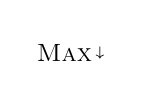
\begin{tikzpicture}[xscale=0.6,yscale=0.4]
\node (max) at (0,0) {{\small \textsc{Max}}};
\node (reg) at (0.75,0.5) {{\fns \textalpha}};
\node (arrow) at (0.75,0) {{\tiny $\downarrow$}};
\node (Rt) at (0.75,-0.5) {{\fns \textbeta}};
\end{tikzpicture}
\end{minipage}
}

\newcommand{\DepAB}{
\begin{minipage}{0.09\textwidth}
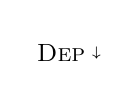
\begin{tikzpicture}[xscale=0.6,yscale=0.4]
\node (max) at (0,0) {{\small \textsc{Dep}}};
\node (reg) at (0.75,0.5) {{\fns \textalpha}};
\node (arrow) at (0.75,0) {{\tiny $\downarrow$}};
\node (Rt) at (0.75,-0.5) {{\fns \textbeta}};
\end{tikzpicture}
\end{minipage}
}

\newcommand{\DepHReg}{
\begin{minipage}{0.055\textwidth}
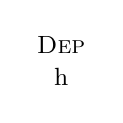
\begin{tikzpicture}[xscale=0.6,yscale=0.4]
\node (dep) at (0,0) {{\small \textsc{Dep}}};
\node (reg) at (0,-1.0) {{\small h}};
\end{tikzpicture}
\end{minipage}
}

\newcommand{\DepLReg}{
\begin{minipage}{0.055\textwidth}

\begin{tikzpicture}[xscale=0.6,yscale=0.4]
\node (dep) at (0,0) {{\small \textsc{Dep}}};
\node (reg) at (0,-1.0) {{\small l}};
\end{tikzpicture}
\end{minipage}
}

\newcommand{\DepReg}{
\begin{minipage}{0.055\textwidth}

\begin{tikzpicture}[xscale=0.6,yscale=0.4]
\node (dep) at (0,0) {{\small \textsc{Dep}}};
\node (reg) at (0,-1.0) {{\small \textrho}};
\end{tikzpicture}
\end{minipage}
}

\newcommand{\DepTRt}{
\begin{minipage}{0.1\textwidth}
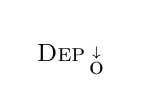
\begin{tikzpicture}[xscale=0.6,yscale=0.4]
\node (dep) at (0,0) {{\small \textsc{Dep}}};
\node (t) at (0.75,0.5) {{\fns \texttau}};
\node (arrow) at (0.75,0) {{\tiny $\downarrow$}};
\node (Rt) at (0.75,-0.5) {{\fns o}};
\end{tikzpicture}
\end{minipage}
}

\newcommand{\MaxRegRt}{
\begin{minipage}{0.1\textwidth}
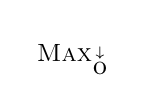
\begin{tikzpicture}[xscale=0.6,yscale=0.4]
\node (max) at (0,0) {{\small \textsc{Max}}};
\node (arrow) at (0.75,0) {{\tiny $\downarrow$}};
\node (Rt) at (0.75,-0.5) {{\fns o}};
\node (reg) at (0.75,0.5) {{\fns \textrho}};
\end{tikzpicture}
\end{minipage}
}

\newcommand{\RegToneByRt}{
\begin{minipage}{0.06\textwidth}
\begin{tikzpicture}[xscale=0.6,yscale=0.5]
\node[rotate=20] (arrow1) at (-0.15,0) {{\fns $\uparrow$}};
\node[rotate=340] (arrow2) at (0.15,0) {{\fns $\uparrow$}};
\node (Rt) at (0,-0.55) {{\small o}};
\node (reg) at (0.4,0.55) {{\small \textrho}};
\node (tone) at (-0.4,0.55) {{\small \texttau}};
\end{tikzpicture}
\end{minipage}
}

\newcommand{\RegToneBySyl}{
\begin{minipage}{0.06\textwidth}
\begin{tikzpicture}[xscale=0.6,yscale=0.5]
\node[rotate=20] (arrow1) at (-0.15,0) {{\fns $\uparrow$}};
\node[rotate=340] (arrow2) at (0.15,0) {{\fns $\uparrow$}};
\node (Rt) at (0,-0.55) {{\small \textsigma}};
\node (reg) at (0.4,0.55) {{\small \textrho}};
\node (tone) at (-0.4,0.55) {{\small \texttau}};
\end{tikzpicture}
\end{minipage}
}

\newcommand{\DepTone}{
\begin{minipage}{0.055\textwidth}

\begin{tikzpicture}[xscale=0.6,yscale=0.4]
\node (dep) at (0,0) {{\small \textsc{Dep}}};
\node (tone) at (0,-1.0) {{\small \texttau}};
\end{tikzpicture}
\end{minipage}
}

\newcommand{\DepTonalRt}{
\begin{minipage}{0.055\textwidth}

\begin{tikzpicture}[xscale=0.6,yscale=0.4]
\node (dep) at (0,0) {{\small \textsc{Dep}}};
\node (tone) at (0,-1.0) {{\small o}};
\end{tikzpicture}
\end{minipage}
}

\newcommand{\DepL}{
\begin{minipage}{0.055\textwidth}

\begin{tikzpicture}[xscale=0.6,yscale=0.4]
\node (dep) at (0,0) {{\small \textsc{Dep}}};
\node (tone) at (0,-1.0) {{\small L}};
\end{tikzpicture}
\end{minipage}
}

\newcommand{\DepH}{
\begin{minipage}{0.055\textwidth}

\begin{tikzpicture}[xscale=0.6,yscale=0.4]
\node (dep) at (0,0) {{\small \textsc{Dep}}};
\node (tone) at (0,-1.0) {{\small H}};
\end{tikzpicture}
\end{minipage}
}

\newcommand{\NoMultDiff}{{\small *loh}}
\newcommand{\Alt}{{\small \textsc{Alt}}}
\newcommand{\NoSkip}{{\small \scell{\textsc{No}\\\textsc{Skip}}}}


\newcommand{\RegDomRt}{
\begin{minipage}{0.030\textwidth}
\begin{tikzpicture}[xscale=0.6,yscale=0.5]
\node (arrow) at (0,0) {{\fns $\downarrow$}};
\node (Rt) at (0,-0.55) {{\small o}};
\node (reg) at (0,0.55) {{\small \textrho}};
\end{tikzpicture}
\end{minipage}
}

\newcommand{\DepRegRt}{
\begin{minipage}{0.1\textwidth}
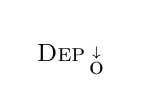
\begin{tikzpicture}[xscale=0.6,yscale=0.4]
\node (dep) at (0,0) {{\small \textsc{Dep}}};
\node (arrow) at (0.75,0) {{\tiny $\downarrow$}};
\node (Rt) at (0.75,-0.5) {{\fns o}};
\node (reg) at (0.75,0.5) {{\fns \textrho}};
\end{tikzpicture}
\end{minipage}
}

% unused

\newcommand{\ToneByRt}{
\begin{minipage}{0.05\textwidth}
\begin{tikzpicture}[xscale=0.6,yscale=0.5]
\node (arrow) at (0,0) {{\fns $\uparrow$}};
\node (Rt) at (0,-0.55) {{\small o}};
\node (tone) at (0,0.55) {{\small \texttau}};
\end{tikzpicture}
\end{minipage}
}

\newcommand{\RegByRt}{
\begin{minipage}{0.05\textwidth}
\begin{tikzpicture}[xscale=0.6,yscale=0.5]
\node (arrow) at (0,0) {{\fns $\uparrow$}};
\node (Rt) at (0,-0.55) {{\small o}};
\node (reg) at (0,0.55) {{\small \textrho}};
\end{tikzpicture}
\end{minipage}
}

\newcommand{\ToneDomRt}{
\begin{minipage}{0.05\textwidth}
\begin{tikzpicture}[xscale=0.6,yscale=0.5]
\node (arrow) at (0,0) {{\fns $\downarrow$}};
\node (Rt) at (0,-0.55) {{\small o}};
\node (tone) at (0,0.55) {{\small \texttau}};
\end{tikzpicture}
\end{minipage}
}

% --- OT tableaus --- %

% Sec. 3.2, first tabl.

\newcommand{\OTHLInput}{
\begin{minipage}{0.17\textwidth}
\begin{tikzpicture}[xscale=\myscalex,yscale=\myscaley]
\node (tone) at (2,0) {(= H)};
\node (syl) at (0,0) {\textsigma};
\node (Rt) at (0,1) {o};
\node (H) at (-0.5,2) {H};
\node (R) at (0.5,3) {h};
\node (Rt2) at (1.5,1.0) {o};
%\node (H2) at (1.0,2) {\epen{L}};
\node (R2) at (2.0,3) {\blue{l}};
\draw [thick] (syl.north) -- (Rt.south) ;
\draw [thick] (Rt.north) -- (H.south) ;
\draw [thick] (Rt.north) -- (R.south) ;
\draw [thick] (syl.north) -- (Rt2.south) ;
%\draw [dashed] (Rt2.north) -- (H2.south) ;
%\draw [dashed] (Rt2.north) -- (R2.south) ;
\end{tikzpicture}
\end{minipage}
}

\newcommand{\OTHLWinner}{
\begin{minipage}{0.17\textwidth}
\begin{tikzpicture}[xscale=\myscalex,yscale=\myscaley]
\node (tone) at (2,0) {(= HL)};
\node (syl) at (0,0) {\textsigma};
\node (Rt) at (0,1) {o};
\node (H) at (-0.5,2) {H};
\node (R) at (0.5,3) {h};
\node (Rt2) at (1.5,1.0) {o};
\node (H2) at (1.0,2) {\epen{L}};
\node (R2) at (2.0,3) {\blue{l}};
\draw [thick] (syl.north) -- (Rt.south) ;
\draw [thick] (Rt.north) -- (H.south) ;
\draw [thick] (Rt.north) -- (R.south) ;
\draw [thick] (syl.north) -- (Rt2.south) ;
\draw [dashed] (Rt2.north) -- (H2.south) ;
\draw [dashed] (Rt2.north) -- (R2.south) ;
\end{tikzpicture}
\end{minipage}
}

\newcommand{\OTHLSpreadingHOnly}{
\begin{minipage}{0.17\textwidth}
\begin{tikzpicture}[xscale=\myscalex,yscale=\myscaley]
\node (tone) at (2,0) {(= HM)};
\node (syl) at (0,0) {\textsigma};
\node (Rt) at (0,1) {o};
\node (H) at (-0.5,2) {H};
\node (R) at (0.5,3) {h};
\node (Rt2) at (1.5,1.0) {o};
%\node (H2) at (1.0,2) {\epen{L}};
\node (R2) at (2.0,3) {\blue{l}};
\draw [thick] (syl.north) -- (Rt.south) ;
\draw [thick] (Rt.north) -- (H.south) ;
\draw [thick] (Rt.north) -- (R.south) ;
\draw [thick] (syl.north) -- (Rt2.south) ;
\draw [dashed] (Rt2.north) -- (R2.south) ;
\draw [dashed] (Rt2.north) -- (H.south) ;
\end{tikzpicture}
\end{minipage}
}

\newcommand{\OTHLInsertH}{
\begin{minipage}{0.17\textwidth}
\begin{tikzpicture}[xscale=\myscalex,yscale=\myscaley]
\node (tone) at (2,0) {(= HM)};
\node (syl) at (0,0) {\textsigma};
\node (Rt) at (0,1) {o};
\node (H) at (-0.5,2) {H};
\node (R) at (0.5,3) {h};
\node (Rt2) at (1.5,1.0) {o};
\node (H2) at (1.0,2) {\epen{H}};
\node (R2) at (2.0,3) {\blue{l}};
\draw [thick] (syl.north) -- (Rt.south) ;
\draw [thick] (Rt.north) -- (H.south) ;
\draw [thick] (Rt.north) -- (R.south) ;
\draw [thick] (syl.north) -- (Rt2.south) ;
\draw [dashed] (Rt2.north) -- (H2.south) ;
\draw [dashed] (Rt2.north) -- (R2.south) ;
\end{tikzpicture}
\end{minipage}
}

\newcommand{\OTHLOverwriting}{
\begin{minipage}{0.17\textwidth}
\begin{tikzpicture}[xscale=\myscalex,yscale=\myscaley]
\node (syl) at (0,0) {\textsigma};
\node (Rt) at (0,1) {o};
\node (H) at (-0.5,2) {H};
\node (R) at (0.5,3) {h};
\node (Rt2) at (1.5,1.0) {o};
%\node (H2) at (1.0,2) {\epen{L}};
\node (R2) at (2.0,3) {\blue{l}};
\draw [thick] (syl.north) -- (Rt.south) ;
\draw [thick] (Rt.north) -- (H.south) ;
\draw [thick] (Rt.north) -- (R.south) ;
\draw [thick] (syl.north) -- (Rt2.south) ;
%\draw [dashed] (Rt2.north) -- (H2.south) ;
\draw [dashed] (Rt.north) -- (R2.south) ;
\node (del) at (0.3,1.9) {\textbf{=}};
\end{tikzpicture}
\end{minipage}
}

\newcommand{\OTHLSpreading}{
\begin{minipage}{0.17\textwidth}
\begin{tikzpicture}[xscale=\myscalex,yscale=\myscaley]
\node (syl) at (0,0) {\textsigma};
\node (Rt) at (0,1) {o};
\node (H) at (-0.5,2) {H};
\node (R) at (0.5,3) {h};
\node (Rt2) at (1.5,1.0) {o};
%\node (H2) at (1.0,2) {\epen{L}};
\node (R2) at (2.0,3) {\blue{l}};
\draw [thick] (syl.north) -- (Rt.south) ;
\draw [thick] (Rt.north) -- (H.south) ;
\draw [thick] (Rt.north) -- (R.south) ;
\draw [thick] (syl.north) -- (Rt2.south) ;
%\draw [dashed] (Rt2.north) -- (H2.south) ;
\draw [dashed] (Rt2.north) -- (H.south) ;
\draw [dashed] (Rt2.north) -- (R.south) ;
\end{tikzpicture}
\end{minipage}
}

% Sec. 4.2, second tabl.: phrase-medial position

\newcommand{\OTHnoLInput}{
\begin{minipage}{0.17\textwidth}
\begin{tikzpicture}[xscale=\myscalex,yscale=\myscaley]
\node (tone) at (2,0) {(= H)};
\node (syl) at (0,0) {\textsigma};
\node (Rt) at (0,1) {o};
\node (H) at (-0.5,2) {H};
\node (R) at (0.5,3) {h};
\node (Rt2) at (1.5,1.0) {o};
%\node (H2) at (1.0,2) {\epen{L}};
%\node (R2) at (2.0,3) {\blue{l}};
\draw [thick] (syl.north) -- (Rt.south) ;
\draw [thick] (Rt.north) -- (H.south) ;
\draw [thick] (Rt.north) -- (R.south) ;
\draw [thick] (syl.north) -- (Rt2.south) ;
\end{tikzpicture}
\end{minipage}
}

\newcommand{\OTHnoLEpenth}{
\begin{minipage}{0.17\textwidth}
\begin{tikzpicture}[xscale=\myscalex,yscale=\myscaley]
\node (tone) at (2,0) {(= HM)};
\node (syl) at (0,0) {\textsigma};
\node (Rt) at (0,1) {o};
\node (H) at (-0.5,2) {H};
\node (R) at (0.5,3) {h};
\node (Rt2) at (1.5,1.0) {o};
\node (H2) at (1.0,2) {\epen{L}};
\node (R2) at (2.0,3) {\epen{h}};
\draw [thick] (syl.north) -- (Rt.south) ;
\draw [thick] (Rt.north) -- (H.south) ;
\draw [thick] (Rt.north) -- (R.south) ;
\draw [thick] (syl.north) -- (Rt2.south) ;
\draw [dashed] (Rt2.north) -- (H2.south) ;
\draw [dashed] (Rt2.north) -- (R2.south) ;
\end{tikzpicture}
\end{minipage}
}

\newcommand{\OTHnoLSpreading}{
\begin{minipage}{0.17\textwidth}
\begin{tikzpicture}[xscale=\myscalex,yscale=\myscaley]
\node (tone) at (2,0) {(= HH)};
\node (syl) at (0,0) {\textsigma};
\node (Rt) at (0,1) {o};
\node (H) at (-0.5,2) {H};
\node (R) at (0.5,3) {h};
\node (Rt2) at (1.5,1.0) {o};
%\node (H2) at (1.0,2) {\epen{L}};
%\node (R2) at (2.0,3) {\blue{l}};
\draw [thick] (syl.north) -- (Rt.south) ;
\draw [thick] (Rt.north) -- (H.south) ;
\draw [thick] (Rt.north) -- (R.south) ;
\draw [thick] (syl.north) -- (Rt2.south) ;
\draw [dashed] (Rt2.north) -- (H.south) ;
\draw [dashed] (Rt2.north) -- (R.south) ;
\end{tikzpicture}
\end{minipage}
}

% Sec. 4.2, third tabl., LM is unaffected by L\%

\newcommand{\OTLMInput}{
\begin{minipage}{0.2\textwidth}
\begin{tikzpicture}[xscale=\myscalex,yscale=\myscaley]
\node (tone) at (2,0) {(= LM)};
\node (syl) at (0,0) {\textsigma};
\node (Rt) at (0,1) {o};
\node (H) at (-0.5,2) {L};
\node (R) at (0.5,3) {l};
\node (Rt2) at (1.5,1.0) {o};
\node (H2) at (1.0,2) {L};
\node (R2) at (2.0,3) {h};
\node (R3) at (3.0,3) {\blue{l}};
\draw [thick] (syl.north) -- (Rt.south) ;
\draw [thick] (Rt.north) -- (H.south) ;
\draw [thick] (Rt.north) -- (R.south) ;
\draw [thick] (syl.north) -- (Rt2.south) ;
\draw [thick] (Rt2.north) -- (H2.south) ;
\draw [thick] (Rt2.north) -- (R2.south) ;
\end{tikzpicture}
\end{minipage}
}

\newcommand{\OTLMReplace}{
\begin{minipage}{0.2\textwidth}
\begin{tikzpicture}[xscale=\myscalex,yscale=\myscaley]
\node (tone) at (2,0) {(= LL)};
\node (syl) at (0,0) {\textsigma};
\node (Rt) at (0,1) {o};
\node (H) at (-0.5,2) {L};
\node (R) at (0.5,3) {l};
\node (Rt2) at (1.5,1.0) {o};
\node (H2) at (1.0,2) {L};
\node (R2) at (2.0,3) {h};
\node (R3) at (3.0,3) {\blue{l}};
\draw [thick] (syl.north) -- (Rt.south) ;
\draw [thick] (Rt.north) -- (H.south) ;
\draw [thick] (Rt.north) -- (R.south) ;
\draw [thick] (syl.north) -- (Rt2.south) ;
\draw [thick] (Rt2.north) -- (H2.south) ;
\draw [thick] (Rt2.north) -- (R2.south) ;
\draw [dashed] (Rt2.north) -- (R3.south) ;
\node (del) at (1.8,2.1) {\textbf{=}};
\end{tikzpicture}
\end{minipage}
}

\newcommand{\OTLMTwoReg}{
\begin{minipage}{0.2\textwidth}
\begin{tikzpicture}[xscale=\myscalex,yscale=\myscaley]
\node (tone) at (2,0) {(= LML)};
\node (syl) at (0,0) {\textsigma};
\node (Rt) at (0,1) {o};
\node (H) at (-0.5,2) {L};
\node (R) at (0.5,3) {l};
\node (Rt2) at (1.5,1.0) {o};
\node (H2) at (1.0,2) {L};
\node (R2) at (2.0,3) {h};
\node (R3) at (3.0,3) {\blue{l}};
\draw [thick] (syl.north) -- (Rt.south) ;
\draw [thick] (Rt.north) -- (H.south) ;
\draw [thick] (Rt.north) -- (R.south) ;
\draw [thick] (syl.north) -- (Rt2.south) ;
\draw [thick] (Rt2.north) -- (H2.south) ;
\draw [thick] (Rt2.north) -- (R2.south) ;
\draw [dashed] (Rt2.north) -- (R3.south) ;
\end{tikzpicture}
\end{minipage}
}

% Sec. 4.2, fourth tabl., L is affected by L\% but M is not

\newcommand{\OTLInput}{
\begin{minipage}{0.17\textwidth}
\begin{tikzpicture}[xscale=\myscalex,yscale=\myscaley]
\node (tone) at (2,0) {(= L)};
\node (syl) at (0,0) {\textsigma};
\node (Rt) at (0,1) {o};
\node (H) at (-0.5,2) {L};
\node (R) at (0.5,3) {l};
\node (R2) at (2,3) {\blue{l}};
\draw [thick] (syl.north) -- (Rt.south) ;
\draw [thick] (Rt.north) -- (H.south) ;
\draw [thick] (Rt.north) -- (R.south) ;
\end{tikzpicture}
\end{minipage}
}

\newcommand{\OTLLowered}{
\begin{minipage}{0.17\textwidth}
\begin{tikzpicture}[xscale=\myscalex,yscale=\myscaley]
\node (tone) at (2,0) {(= LL)};
\node (syl) at (0,0) {\textsigma};
\node (Rt) at (0,1) {o};
\node (H) at (-0.5,2) {L};
\node (R) at (0.5,3) {l};
\node (R2) at (2,3) {\blue{l}};
\draw [thick] (syl.north) -- (Rt.south) ;
\draw [thick] (Rt.north) -- (H.south) ;
\draw [thick] (Rt.north) -- (R.south) ;
\draw [dashed] (Rt.north) -- (R2.south) ;
\end{tikzpicture}
\end{minipage}
}

\newcommand{\OTMInput}{
\begin{minipage}{0.17\textwidth}
\begin{tikzpicture}[xscale=\myscalex,yscale=\myscaley]
\node (tone) at (2,0) {(= M)};
\node (syl) at (0,0) {\textsigma};
\node (Rt) at (0,1) {o};
\node (H) at (-0.5,2) {L};
\node (R) at (0.5,3) {h};
\node (R2) at (2,3) {\blue{l}};
\draw [thick] (syl.north) -- (Rt.south) ;
\draw [thick] (Rt.north) -- (H.south) ;
\draw [thick] (Rt.north) -- (R.south) ;
\end{tikzpicture}
\end{minipage}
}

\newcommand{\OTMLowered}{
\begin{minipage}{0.17\textwidth}
\begin{tikzpicture}[xscale=\myscalex,yscale=\myscaley]
\node (tone) at (2,0) {(= ML)};
\node (syl) at (0,0) {\textsigma};
\node (Rt) at (0,1) {o};
\node (H) at (-0.5,2) {L};
\node (R) at (0.5,3) {h};
\node (R2) at (2,3) {\blue{l}};
\draw [thick] (syl.north) -- (Rt.south) ;
\draw [thick] (Rt.north) -- (H.south) ;
\draw [thick] (Rt.north) -- (R.south) ;
\draw [dashed] (Rt.north) -- (R2.south) ;
\end{tikzpicture}
\end{minipage}
}

% Sec. 4.2, fifth tableau, polar questions with level tones

\newcommand{\OTLPolIn}{
\begin{minipage}{0.20\textwidth}
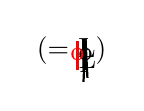
\begin{tikzpicture}[xscale=\myscalex-0.05,yscale=\myscaley-0.05]
\node (tone) at (3.5,0) {(= L)};
\node (syl) at (0,0) {\textsigma};
\node (syl2) at (2,0) {\red{\textsigma}};
\node (Rt) at (0,1) {o};
\node (H) at (-0.5,2) {L};
\node (R) at (0.5,3) {l};
\node (Rt2) at (2,1) {\red{o}};
\draw [thick] (syl.north) -- (Rt.south) ;
\draw [thick,red] (syl2.north) -- (Rt2.south) ;
\draw [thick] (Rt.north) -- (H.south) ;
\draw [thick] (Rt.north) -- (R.south) ;
\end{tikzpicture}
\end{minipage}
}

\newcommand{\OTLPolDef}{
\begin{minipage}{0.20\textwidth}
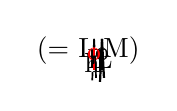
\begin{tikzpicture}[xscale=\myscalex-0.05,yscale=\myscaley-0.05]
\node (tone) at (3.5,0) {(= L.M)};
\node (syl) at (0,0) {\textsigma};
\node (syl2) at (2,0) {\red{\textsigma}};
\node (Rt) at (0,1) {o};
\node (H) at (-0.5,2) {L};
\node (R) at (0.5,3) {l};
\node (H2) at (1.5,2) {\epen{L}};
\node (R2) at (2.5,3) {\epen{h}};
\node (Rt2) at (2,1) {\red{o}};
\draw [thick] (syl.north) -- (Rt.south) ;
\draw [thick,red] (syl2.north) -- (Rt2.south) ;
\draw [thick] (Rt.north) -- (H.south) ;
\draw [thick] (Rt.north) -- (R.south) ;
\draw [semithick,dashed] (Rt2.north) -- (H2.south) ;
\draw [semithick,dashed] (Rt2.north) -- (R2.south) ;
\end{tikzpicture}
\end{minipage}
}

\newcommand{\OTLPolAlt}{
\begin{minipage}{0.20\textwidth}
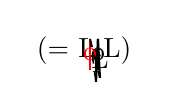
\begin{tikzpicture}[xscale=\myscalex-0.05,yscale=\myscaley-0.05]
\node (tone) at (3.5,0) {(= L.L)};
\node (syl) at (0,0) {\textsigma};
\node (syl2) at (2,0) {\red{\textsigma}};
\node (Rt) at (0,1) {o};
\node (H) at (-0.5,2) {L};
\node (R) at (0.5,3) {l};
\node (Rt2) at (2,1) {\red{o}};
\draw [thick] (syl.north) -- (Rt.south) ;
\draw [thick,red] (syl2.north) -- (Rt2.south) ;
\draw [thick] (Rt.north) -- (H.south) ;
\draw [thick] (Rt.north) -- (R.south) ;
\draw [semithick,dashed] (Rt2.north) -- (H.south) ;
\draw [semithick,dashed] (Rt2.north) -- (R.south) ;
\end{tikzpicture}
\end{minipage}
}

% Sec. 4.2, sixth tableau, polar questions with contour tones

\newcommand{\OTLLPolIn}{
\begin{minipage}{0.23\textwidth}
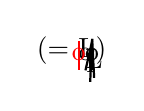
\begin{tikzpicture}[xscale=\myscalex-0.05,yscale=\myscaley-0.05]
\node (tone) at (5.2,0) {(= L)};
\node (syl) at (0,0) {\textsigma};
\node (syl3) at (3.4,0) {\red{\textsigma}};
\node (Rt) at (0,1) {o};
\node (Rt2) at (1.7,1) {o};
\node (Rt3) at (3.4,1) {\red{o}};
\node (H) at (-0.5,2) {L};
\node (R) at (0.5,3) {l};
\draw [thick] (syl.north) -- (Rt.south) ;
\draw [thick] (syl.north) -- (Rt2.south) ;
\draw [thick,red] (syl3.north) -- (Rt3.south) ;
\draw [thick] (Rt.north) -- (H.south) ;
\draw [thick] (Rt.north) -- (R.south) ;
\end{tikzpicture}
\end{minipage}
}

\newcommand{\OTLLPolDef}{
\begin{minipage}{0.23\textwidth}
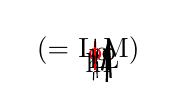
\begin{tikzpicture}[xscale=\myscalex-0.05,yscale=\myscaley-0.05]
\node (tone) at (5.2,0) {(= L.M)};
\node (syl) at (0,0) {\textsigma};
\node (syl3) at (3.4,0) {\red{\textsigma}};
\node (Rt) at (0,1) {o};
\node (Rt2) at (1.7,1) {o};
\node (Rt3) at (3.4,1) {\red{o}};
\node (H) at (-0.5,2) {L};
\node (R) at (0.5,3) {l};
\node (H3) at (2.9,2) {\epen{L}};
\node (R3) at (3.9,3) {\epen{h}};
\draw [thick] (syl.north) -- (Rt.south) ;
\draw [thick] (syl.north) -- (Rt2.south) ;
\draw [thick,red] (syl3.north) -- (Rt3.south) ;
\draw [thick] (Rt.north) -- (H.south) ;
\draw [thick] (Rt.north) -- (R.south) ;
\draw [dashed] (Rt3.north) -- (H3.south) ;
\draw [dashed] (Rt3.north) -- (R3.south) ;
\end{tikzpicture}
\end{minipage}
}

\newcommand{\OTLLPolSkip}{
\begin{minipage}{0.23\textwidth}
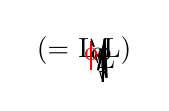
\begin{tikzpicture}[xscale=\myscalex-0.05,yscale=\myscaley-0.05]
\node (tone) at (5.2,0) {(= L.L)};
\node (syl) at (0,0) {\textsigma};
\node (syl3) at (3.4,0) {\red{\textsigma}};
\node (Rt) at (0,1) {o};
\node (Rt2) at (1.7,1) {o};
\node (Rt3) at (3.4,1) {\red{o}};
\node (H) at (-0.5,2) {L};
\node (R) at (0.5,3) {l};
\draw [thick] (syl.north) -- (Rt.south) ;
\draw [thick] (syl.north) -- (Rt2.south) ;
\draw [thick,red] (syl3.north) -- (Rt3.south) ;
\draw [thick] (Rt.north) -- (H.south) ;
\draw [thick] (Rt.north) -- (R.south) ;
\draw [dashed] (Rt3.north) -- (H.south) ;
\draw [dashed] (Rt3.north) -- (R.south) ;
\end{tikzpicture}
\end{minipage}
}  
  
\newcommand{\ilit}[1]{#1\il{#1}}    
\newcommand{\isit}[1]{#1\is{#1}}  

\makeatletter
\let\thetitle\@title
\let\theauthor\@author 
\makeatother

\newcommand{\togglepaper}[1][0]{ 
  \bibliography{../localbibliography}
  %% hyphenation points for line breaks
%% Normally, automatic hyphenation in LaTeX is very good
%% If a word is mis-hyphenated, add it to this file
%%
%% add information to TeX file before \begin{document} with:
%% %% hyphenation points for line breaks
%% Normally, automatic hyphenation in LaTeX is very good
%% If a word is mis-hyphenated, add it to this file
%%
%% add information to TeX file before \begin{document} with:
%% \include{localhyphenation}
\hyphenation{
affri-ca-te
affri-ca-tes
com-ple-ments
par-a-digm
Sha-ron
Kings-ton
phe-nom-e-non
Daul-ton
Abu-ba-ka-ri
Ngo-nya-ni
Clem-ents 
King-ston
Tru-cken-brodt
Tab-leau
cophono-logies
mark-edness
Ti-gri-nya
a-mong
Car-stens
Lu-bu-ku-su
}
\hyphenation{
affri-ca-te
affri-ca-tes
com-ple-ments
par-a-digm
Sha-ron
Kings-ton
phe-nom-e-non
Daul-ton
Abu-ba-ka-ri
Ngo-nya-ni
Clem-ents 
King-ston
Tru-cken-brodt
Tab-leau
cophono-logies
mark-edness
Ti-gri-nya
a-mong
Car-stens
Lu-bu-ku-su
}
  \papernote{\scriptsize\normalfont
    \theauthor.
    \thetitle. 
    To appear in: 
    Emily Clem,   Peter Jenks \& Hannah Sande.
    Theory and description in African Linguistics: Selected papers from the 47th Annual Conference on African Linguistics.
    Berlin: Language Science Press. [preliminary page numbering]
  }
  \pagenumbering{roman}
  \setcounter{chapter}{#1}
  \addtocounter{chapter}{-1}
}

\newcommand{\upstep}{\textupstep}


% \newcounter{tableauxcounter}

\renewcommand{\textltailn}{ɲ}
\renewcommand{\textbardotlessj}{ɟ}

\newcommand{\emphkh}[1]{\textit{#1}} %originally \textbf, banned by the guidelines



\definecolor{lsDOIGray}{cmyk}{0,0,0,0.45}


\newcommand{\xuparrow}[1]{%
  {\left\uparrow\vbox to #1{}\right.\kern-\nulldelimiterspace}
}
\renewcommand \textupstep[1]{\char"A71B#1}
\renewcommand \textdownstep[1]{\char"A71C#1}
 
 \newcommand{\ꜛ}{\textsf{ꜛ}}
 
\def\biberror{\undefined}


\newcommand{\OTbox}[1]{\resizebox{.88\textwidth}{!}{#1}}
 
\usepackage{pifont.sty}

% TODO Fll this in
\author{Lee Bickmore\affiliation{University at Albany, SUNY}}
\title{Liquid realization in Rutooro}
\abstract{This paper provides a description and analysis of te distribution of the liquids [r] and [l] in Rutooro (E.12), a Ugandan Bantu language. The allophone that appears is conditioned by the backness of both the preceding and following vowel. Assuming /r/ is underlying, it changes to [l] in contexts when the preceding vowel is back and the following vowel is front. A systematic set of apparent surface counter-examples, leading to phrasal minimal pairs, are argued to be the result of the rule applying twice -- both lexically and post lexically, where a separate post-lexical rule of vowel deletion is responsible for the opacity.}
\begin{document}
\maketitle
\section{Introduction}

\ili{Rutooro} (E/J.12) is a \ili{Bantu} language spoken by roughly a half million speakers in western Uganda. Other closely related languages in the “Nyooro/Ganda” group include: \ili{Luganda}, Runyankore, Ruciga, Nyooro, Soga, and \ili{Gwere}. Previous work on the language includes a dictionary \citep{Kaji2007} a brief article on the \isi{tone} \citep{Kaji2008}, and a Runyooro-\ili{Rutooro} grammar \citep{Rubongoya1999}. The data presented in this paper were collected from Barbara Balinda, a 26 year old native speaker from Fort Portal, currently residing in Albany, NY.

The goal of this paper is to describe and analyze the distribution of \isi{liquid} consonants in \ili{Rutooro}. It will be argued that the lateral [l], the flap [ɾ], and the trilled [r] are all allophones of a single underlying sound. While the realization of the trill is fairly straightforward to characterize, the \isi{complementary distribution} between the lateral and flap is much more complex, and is the \isi{focus} of this study. First, the distribution of these two allophones within single words is such that it is not immediately obvious which should be characterized as the elsewhere case and therefore chosen to be basic. Only after examining \isi{liquid} realization within phrases is it evident which of these must be posited as underlying. Second, whichever is chosen to be basic, the derivation of the other must include information about both the preceding and following vowels. Third, given the triggering environment, it does not appear that this process can be considered one of assimilation. Finally, while \citet{Kaji2008} provides a solid description of the \isi{complementary distribution} among these three allophones (completely consistent with what I found), it is based solely on word-level data. This study significantly expands our understanding of the realization of these sounds by considering phrasal data. Accounting for this allophony in a rule-based approach, it will be argued that the rule affecting a change in [lateral] actually has two chances to apply: once at the word level and again at the phrasal level. This cyclic-type ordering actually leads to phrasal minimal pairs involving the two liquids, even though they are not underlyingly contrastive.

\section{Distribution of liquid consonants}
\subsection{Liquid realization at the word level}

Phonetically, there are three \isi{liquid} consonants in \ili{Rutooro}: the lateral [l], the flap [ɾ] and the trilled [r], all in \isi{complementary distribution}. (The articulation of the [r], while a trill in the speech of some \ili{Rutooro} spreakers, is realized as an alveolar approximate in that of others.) The practical orthography of the language represents the \isi{liquid} as <l>, the flap as <r> and the trill as <rr>. I will use this more orthographic representation of these three sounds from here forward. In addition, while I will suggest below that it is not in fact immediately obvious whether the underlying segment should be posited as /l/ or /r/, evidence discussed later suggests it should be /r/. I assume that here and will defend it in \sectref{sec:bickmore:2.3}.\footnote{With regard to the \ili{Rutooro} transcriptions, no \isi{tone} is marked. \ili{Rutooro} is one of the relatively few \ili{Bantu} languages where all lexical \isi{tone} contrast has been lost. Synchronically, a High is predictably found on the penult of each \isi{phonological phrase}.}%
%Footnote added in response to reviewer’s question about \isi{tone}. 
%

The trilled \isi{liquid} is the phonetic realization of two underlying /r/s becoming adjacent due to a process that deletes a vowel (most commonly /i/) between them. This can be seen in the examples below.

\ea\label{ex:bickmore:1}
\ea\label{ex:bickmore:1a}
\glll omu-rro \\
/omu-riro/\\
C3-fire\\
\glt ‘fire’\\
\ex\label{ex:bickmore:1b}
\glll ku-rr-a \\
/ku-rir-a/\\
\textsc{inf-}\textup{cry}\textsc{{}-fv}\\
\glt  ‘to cry’\\
\ex\label{ex:bickmore:1c}
\glll ba-kor-r-e \\
/ba-kor-ir-e/\\
\textsc{3pl-}\textup{work}\textsc{{}-appl-fv}\\
\glt  ‘that they work for’\\
\z
\z
%
%While I appreciate the reviewer’s comments here, I’m not sure it’s appropriate to address them in the paper. As the reviewer notes, if one assumes deletion before the r>l change, these are not problematic. But it doesn’t make sense to say that here before the r>l rule is even presented. I guess I could add a footnote later, but I just don’t see this as a major issue for the reader.
%Also, it’s just not the case that all the /r/s  in (1) have preceding back vowels. The vowel preceding the second /r/ in both 1b and 1c is front.
%

I will now show that the distribution of the lateral and flap allophones of /r/ depends upon both what immediately precedes and follows the \isi{liquid}. Specifically, it is the backness of any adjacent vowels which condition the distribution. The lateral is found when two conditions %
%Again, while it’s true that the \ili{Luganda} r/l allophony is well{}-known, I just don’t think mentioning it here is necessarily relevant or helpful. The distribution in \ili{Rutooro} is completely different, plus if one is going to mention \ili{Luganda}, then why not other related languages. While I’m a huge fan of historical/comparative analyses, that’s not the \isi{focus} of this paper.
%
are met: 1) it is word-initial or preceded by a back vowel, and 2) it is followed by a front vowel. This is illustrated in the examples from nouns below (where the hyphen separates the nominal class prefix and the stem).

\ea\label{ex:bickmore:2}
[l] in  [+bk] \underline{ }\underline{ } [-bk]
\ea\label{ex:bickmore:2a}
\downingdouble{omu-gole}{‘bride’}
\ex\label{ex:bickmore:2b}
\downingdouble{oru-baale}{‘hail’}
\ex\label{ex:bickmore:2c}
\downingdouble{e-gali}{‘bicycle’}
\ex\label{ex:bickmore:2d}
\downingdouble{eki-cooli}{‘corn’}
\z
\z

\ea\label{ex:bickmore:3}
[l] in  [\textsubscript{w} \underline{ }\underline{ } [-bk]
\downingdouble{leesu}{‘waistcloth’}
\z

The \isi{liquid} phoneme is realized as [r] when either: a) followed by a back vowel or b) preceded by a front vowel.

\ea\label{ex:bickmore:4}
[r] in  [+bk] \underline{ }\underline{ } [+bk]
\ea\label{ex:bickmore:4a}
\downingdouble{en-garo}{‘hand’}
\ex\label{ex:bickmore:4b}
\downingdouble{oru-kurato}{‘meeting’}
\ex\label{ex:bickmore:4c}
\downingdouble{aka-tuunguru}{‘onion’}
\ex\label{ex:bickmore:4d}
\downingdouble{en-jora}{‘cloth’}
\z
\z

\ea\label{ex:bickmore:5}
[r] in  [-bk] \underline{ }\underline{ } [+bk]
\ea\label{ex:bickmore:5a}
\downingdouble{bendera}{‘flag’}
\ex\label{ex:bickmore:5b}
\downingdouble{eki-bira}{‘forest’}
\ex\label{ex:bickmore:5c}
\downingdouble{i-somero}{‘school’}
\ex\label{ex:bickmore:5d}
\downingdouble{eki-cumbiro}{‘kitchen’}
\z
\z

\noindent\parbox{\textwidth}{\ea\label{ex:bickmore:6}
[r] in  [\textsubscript{W}%
%I’ll leave the bracket labeling to the editors as they’ll want consistency across papers.
%
 \underline{ }\underline{ } [+bk]
\ea\label{ex:bickmore:6a}
\downingdouble{raangi}{‘color’}
\ex\label{ex:bickmore:6b}
\downingdouble{ruhanga}{‘God’}
\ex\label{ex:bickmore:6c}
\downingdouble{rugabire}{‘sandal’}
\z
\z}

\ea\label{ex:bickmore:7}
[r] in  [-bk] \underline{ }\underline{ } [-bk]
\ea\label{ex:bickmore:7a}
\downingdouble{omu-zaire}{‘parent’}
\ex\label{ex:bickmore:7b}
\downingdouble{eki-gere}{‘foot’}
\ex\label{ex:bickmore:7c}
\downingdouble{firimu}{‘film’}
\ex\label{ex:bickmore:7d}
\downingdouble{omu-ceeri}{‘rice’}
\z
\z

Given the distribution described and illustrated above, neither the environment where [r] is found, nor the one where [l] is found can be stated simply, i.e. without recourse to disjunction. In \REF{ex:bickmore:8} we formulate the rule necessary if /r/ is chosen to be basic, and in \REF{ex:bickmore:9} we formulate the rule necessary if /l/ is chosen to be basic. As can be seen both involve a disjunctive environment, requiring the use of curly brackets. 

% \newcommand{\phonrule}[3]{#1 $\to$ #2 / #3}
% \newcommand{\featurebox}[1]{$\left[\begin{tabular}{>{\scshape}c}#1\end{tabular}\right]$}

\ea\label{ex:bickmore:8}
Assuming /r/ to be underling    \\
$r\to l/
\left\{
\begin{array}{l}
{\db}\#\\{}
[+bk]
\end{array}
\right\}
{\longrule}
[-bk]
$


 
 \z

\ea\label{ex:bickmore:9}
Assuming /l/ to be underling\\
$l\to r/
\left\{
\begin{array}{l}
[-bk]{\longrule}\\
{\longrule}[+bk]
\end{array}
\right\} 
$

 
 
\z


 

While neither the distribution of [l], nor [r] is easily identified as the “elsewhere” case, we will see evidence later which favors the choice of /r/ as the phoneme. Until then, as noted above, I will assume /r/ in the discussion which follows. 

The forms in (\ref{ex:bickmore:2}--\ref{ex:bickmore:6}) show the realization of the \isi{liquid} in contexts where the \isi{liquid} is tautomorphemic with the surrounding vowels. That this allophonic variation can in fact result in morphological alternations is shown in the examples below:

\ea\label{ex:bickmore:10}
Verb roots ending Back Vowel + /r/ 
\ea\label{ex:bickmore:10a}
ku-har-a  ‘to scratch’%
%Footnote 1 was added to address the question of \isi{tone}.
%
\ex\label{ex:bickmore:10b}
\downingdouble{ba-hal-e}{‘that they scratch’}
\ex\label{ex:bickmore:10c}
\downingdouble{ku-zoor-a}{‘to find’}
\ex\label{ex:bickmore:10d}
\downingdouble{ba-zool-e}{‘that they find’}
\ex\label{ex:bickmore:10e}
\downingdouble{ku-sasur-a}{‘to pay’}
\ex\label{ex:bickmore:10f}
\downingdouble{ba-sasul-e}{‘that they pay’}
\z
\z

\ea\label{ex:bickmore:11}
Alternations in class 5 nominal prefix /ri-/ 
\ea\label{ex:bickmore:11a}
\downingdouble{e-ri-ino}{‘tooth’}
\ex\label{ex:bickmore:11b}
\downingdouble{li-ino}{‘it is a tooth’}
\ex\label{ex:bickmore:11c}
\downingdouble{e-ri-iso}{‘eye’}
\ex\label{ex:bickmore:11d}
\downingdouble{li-iso}{‘it is an eye’}
\ex\label{ex:bickmore:11e}
\downingdouble{e-rii-ndazi}{‘doughnut’}
\ex\label{ex:bickmore:11f}
\downingdouble{lii-ndazi}{‘it is a doughnut’}
\z
\z

In \REF{ex:bickmore:10} it can be seen that the root-final \isi{liquid}, preceded by a [+back] vowel, surfaces as [r] before the [+back] default Final Vowel /-a/ (cf. \ref{ex:bickmore:4}), but as [l] before the [-back] subjunctive Final Vowel /-e/ (cf. \ref{ex:bickmore:2}). In \REF{ex:bickmore:11} the \isi{liquid} of the Class 5 noun prefix surfaces as [r] when preceded by the [-back] preprefix /e-/ (cf. \ref{ex:bickmore:7}), but as [l], when no preprefix precedes (cf. \ref{ex:bickmore:3}), signaling the copulative meaning. 

Below, it is shown that [back] value of glides is equally relevant in the determination of the distribution of the \isi{liquid} allophones. 

\ea\label{ex:bickmore:12}
Effect of glides
\ea\label{ex:bickmore:12a}
\downingtriple{ba-sasul-e}{‘that they pay’}{/ba-sasur-e/}
\ex\label{ex:bickmore:12b}
\downingtriple{ba-sasur-w-e}{‘that they be paid’}{/ba-sasur-u-e/}
\ex\label{ex:bickmore:12c}
\downingtriple{ba-zool-e}{‘that they find’}{/ba-zoor-e/}
\ex\label{ex:bickmore:12d}
\downingtriple{ba-zoor-w-e}{‘that they be found’}{/ba-zoor-u-e/}
\ex\label{ex:bickmore:12e}
\downingtriple{ku-gi-ry-a}{‘to eat them (C4)’}{/ku-gi-ri-a/}
\ex\label{ex:bickmore:12f}
\downingtriple{ku-ly-a}{‘to eat’}{/ku-ri-a/}
\ex\label{ex:bickmore:12g}
\downingtriple{e-ry-aato}{‘boat’}{/e-ri-ato/}
\ex\label{ex:bickmore:12h}
\downingtriple{ly-aato}{‘it is a boat’}{/ri-ato/}
\z
\z
%I have in fact represented the passive as a /{}-u/, as in 12b,d. But no, I have not collected the relevant forms with an enclitic to see if you get compensatory lengthening in passives. My guess is that you would, but again, while interesting, I don’t see how this is at all crucial to the point at hand or goals of the paper.
%

The examples in (\ref{ex:bickmore:12a}--\ref{ex:bickmore:12d}) show that the glide [w] acts as a [+back] segment in triggering the realization of this \isi{liquid} phoneme. As the \isi{liquid} is surrounded by two [+back] vocoids in those cases, it surfaces as [r]. The examples in (\ref{ex:bickmore:12e}--\ref{ex:bickmore:12h}) show that the glide [y] acts as a [-back] segment in this regard. Since the \isi{liquid} is word-initial and followed by a [-back] vocoid in those cases, it surfaces as [l]

\subsection{Liquids realization at the phrase level}

Having established the environments that [l] and [r] appear in at the level of the word, let us now turn to phrases. First we consider the short phrases in (\ref{ex:bickmore:13}--\ref{ex:bickmore:15}).

\ea\label{ex:bickmore:13}
\gll  ku-leet-a li-nu  \\
\textsc{inf-}\textup{bring}\textsc{{}-fv} \textsc{c5-dem}\\
\glt  ‘to bring this one (C5)’  
\z

\ea\label{ex:bickmore:14}
\gll  ba-leet-e li-nu  \\
\textsc{3pl-}\textup{bring}\textsc{{}-Subj} \textsc{c5-dem}\\
\glt  ‘that they bring this one (C5)’
\z

\ea\label{ex:bickmore:15}
\gll  e-ki-sani li-ino  \\
\textsc{iv-c7-}\textup{drawing} \textsc{c5-}\textup{tooth}\\
\glt  ‘the drawing is a tooth’    
\z

In (\ref{ex:bickmore:13}--\ref{ex:bickmore:15}) the word-initial (but phrase-medial) Class 5 noun prefix in each case is realized as [l]. We saw this in \REF{ex:bickmore:15} and (\ref{ex:bickmore:11}b,~d,~f) where the \isi{liquid} was followed by a [-back] vowel but not preceded by any sound (being both word and phrase-initial in those cases). However, we have also seen that when the \isi{liquid} is both preceded by and followed by [-back] vowels, as in \REF{ex:bickmore:7} and (\ref{ex:bickmore:11}a,~c,~e), it is realized as [r]. We conclude from the examples in (\ref{ex:bickmore:13}--\ref{ex:bickmore:15}) that it is not possible to simply say that the domain of application of the r → l rule in \REF{ex:bickmore:8} is the phrase (with no regard to word boundaries) as such would ungrammatically predict the realization of [r] in these cases. One way to account for these facts is to posit the r → l rule in \REF{ex:bickmore:8} as a word-level process, taking place before any post-lexical rules. 

Before investigating \isi{liquid} resolution in additional phrasal contexts, we must first examine a process of \isi{vowel deletion} that operates across words. As seen in the phrasal data below, a [-hi] vowel at the end of a word deletes before a following word-initial vowel, with a compensatory lengthening of that second vowel.


\ea\label{ex:bickmore:16}
\ea\label{ex:bickmore:16a}
\glll ku-leet oo-muu-ntu  \\
      /ku-leet-a o-mu-ntu/\\
  \textsc{inf-}\textup{bring}\textsc{{}-fv} \textsc{iv-c1-}\textup{person}\\
\glt      ‘to bring the person’

\ex\label{ex:bickmore:16b}
\glll ku-som ee-ki-tabu\\        
/ku-som-a e-ki-tabu/\\
\textsc{inf-}\textup{read}\textsc{{}-fv} \textsc{iv-c7-}\textup{book}\\
\glt      ‘to read the book’

\ex\label{ex:bickmore:16c}
\glll ba-han aa-baa-ntu\\
/ba-han-e a-ba-ntu/\\
\textsc{3pl-}\textup{advise}\textsc{{}-Subj} \textsc{iv-c2-}\textup{people}\\
\glt      ‘that they advise people’
\z
\z

The rule accounting for this is formalized below:

\ea\label{ex:bickmore:17}
Vowel Deletion%
%Yes. I didn’t include every possible VV combination as that would lengthen the paper unnecessarily.
%

         V → ø / \underline{ }\underline{ }\underline{ } ]\textsubscript{w} \textsubscript{w}[ V  

      [-hi]
\z
Given, this process we can now examine some additional phrases that are relevant to our understanding of \isi{liquid} realization, namely those where an underlying \isi{liquid} precedes a word-\isi{final vowel} that will be deleted by the rule in \REF{ex:bickmore:17}. First let us examine the case where the vowel preceding the \isi{liquid} is [-back], and the first vowel of the following word is [+back]

\ea\label{ex:bickmore:18}
\ea\label{ex:bickmore:18a}
\glll  ba-zool oo-muu-ntu    \\
      /ba-zoor-e o-mu-ntu/	\\
\textsc{3pl-}\textup{find}\textsc{{}-Subj} \textsc{iv-c1-}\textup{person}\\
\glt      ‘that they find the person’
\ex\label{ex:bickmore:18b}
\glll  ba-zool aa-baa-ntu    \\
      /ba-zoor-e a-ba-ntu/	\\
\textsc{3pl-}\textup{find}\textsc{{}-Subj} \textsc{iv-c2-}\textup{person}\\
\glt      ‘that they find the people’
\ex\label{ex:bickmore:18c}
\glll  a-ka-tal aa-ko    \\
      /a-ka-tare a-ko/	\\
\textsc{iv-c13-}\textup{market} \textsc{iv-dem.13}\\
\glt      ‘this market’
\ex\label{ex:bickmore:18d}
\glll  o-bu-zaal oo-bu    \\
      /o-bu-zaare o-bu/	\\
\textsc{iv-c14-kinship} \textsc{iv-dem.14}\\
\glt      ‘that kinship’
\z
\z

In each case above the \isi{liquid} is underlying preceded by a back vowel. While it is followed by a [-back] vowel underlyingly, due to application of Vowel Deletion, it is followed by a [+back] vowel on the surface within the phrase. As can be seen, in each case the \isi{liquid} is realized as [l]. Here again, if were to assume that \isi{liquid} realization is a phrase-level process that occurs after Vowel Deletion, we would incorrectly predict that the \isi{liquid} should surface as [r], as it did in \REF{ex:bickmore:4} between two back vowels. If, however, we consider the \isi{liquid} realization rule to take place at the word level, we directly account for the patterns in \REF{ex:bickmore:18}, as we did in \REF{ex:bickmore:16}. This is illustrated in the derivation below of 18a), where Vowel Deletion counter-bleeds the r → l rule.

\ea\label{ex:bickmore:19}
\downingdouble{/ba-zoor-e o-mu-ntu/}{UR}
\downingdouble{ba-zool-e o-mu-ntu}{r → l (word-level)}
\downingdouble{ba-zool oo-mu-ntu}{V-Deletion (phrase-level)}
\z

Finally, let us examine the case where the vowel preceding the \isi{liquid} is [+back], the word-\isi{final vowel} after it is [-back], and the following word begins with a [+back] vowel.

\ea\label{ex:bickmore:20}
\ea\label{ex:bickmore:20a}
\glll ku-zool ee-bi-tabu\\
      /ku-zool-a e-bi-tabu    \\
\textsc{inf-}\textup{find}\textsc{{}-fv} \textsc{iv-C8-}\textup{book}\\
\glt      ‘to find the books’
\ex\label{ex:bickmore:20b}
\glll  ku-hal ee-bii-ntu    \\
      /ku-har-a e-bi-ntu/	\\
\textsc{inf-}\textup{scratch}\textsc{{}-fv} \textsc{iv-C8-}\textup{thing}\\
\glt      ‘to scratch the things’
\ex\label{ex:bickmore:20c}
\glll e-ky-aal ee-ki    \\
      /e-ki-ara e-ki/	\\
\textsc{iv-C7-}\textup{finger} \textsc{iv-dem.7}\\
\glt      ‘that finger’
\ex\label{ex:bickmore:20d}
\glll e-ki-kool ee-ki    \\
      /e-ki-koora e-ki/	\\
\textsc{iv-C7-}\textup{dry.leaf} \textsc{iv-dem.7}\\
\glt      ‘that dry leaf’
\z
\z

In each case above the \isi{liquid} is realized as [l]. Yet, this is unexpected given our current analysis. If the r → l rule applies at the level of the word, we would expect it not to apply in these cases since the \isi{liquid} within the word is both preceded and followed by a [+back] vowel, an environment where [r] is attested (cf. \ref{ex:bickmore:4}). In order to account for the realization of the \isi{liquid} as the lateral in these phrases, we must assume that the r → l rule applies \textit{after} Vowel Deletion, as it must be fed by it. This is shown in the derivation below of 20a). 

\ea\label{ex:bickmore:21}
\downingdouble{/ku-zoor-a e-bi-tabu/}{UR}
\downingdouble{ku-zoor ee-bii-tabu}{V-Deletion (phrase-level)}
\downingdouble{ku-zool ee-bii-tabu}{r → l (phrase-level)}
\z

Yet, if the r → l rule is only a phrase-level one, it will fail to account for phrases such as the ones in (\ref{ex:bickmore:13}--\ref{ex:bickmore:18}), as detailed above. Within this rule-based derivational framework, one way to account for all of the phrases examined here is to posit the r → l rule as \textit{both} a word-level, as well as a post-lexical phrasal process.%
%While potentially interesting, and while I’ve played around with various OT analysis, I just don’t think it prudent in terms of space or \isi{focus} to introduce even the beginning of one here.
%
 In crude terms, under this analysis an underling /r/ has two chances to become [l]—first if the structural description of the process is met within the word, and again if the structural description is met at the level of the phrase, after \isi{vowel deletion}. 

Next, it is interesting to note that while [r] and [l] are allophonic variations of a single phoneme in \ili{Rutooro}, their complex realization%
%My response to the reviewer’s comment is really the last sentence before section 2.3.  Not sure if I have anything further to add. I agree that r and l can be justified as allophones on the word level. But you do get these minimal pairs at the phrase level.
%
 patterns can actually lead to minimal pairs at the phrase level. This is shown below.

\ea\label{ex:bickmore:22}
\glll    tu-bal aa-maa-ndazi\\
    /tu-bar-e a-ma-ndazi/	\\
\textsc{1pl-}\textup{count}\textsc{{}-Subj} \textsc{iv-C6-}\textup{donut}\\
\glt    ‘let’s count the donuts’
\z

\ea\label{ex:bickmore:23}
\glll    tu-bar-a a-maa-ndazi\\
    /tu-bar-a a-ma-ndazi/	\\
\textsc{1pl-}\textup{count}\textsc{{}-fv} \textsc{iv-C6-}\textup{donut}\\
\glt    ‘we count donuts (Habit)’
\z


The example in \REF{ex:bickmore:22} is in the Subjunctive which is formed by adding the suffix /-e/ onto the verb. The r→l rule will apply at the level of the word as its structural description is met there. Vowel Deletion will eliminate the /-e/ resulting in a compensatorily lengthened [aa] after the \isi{liquid}. The example in \REF{ex:bickmore:23} is in the Habitual which is formed by adding the default Final Vowel /-a/ onto the verb. The r→l rule will not apply at the level of the word as the /l/ is both preceded and followed by a [+back] vowel. This remains true at the phrasal level as well, and thus the \isi{liquid} is realized as [r]. Thus, even though these two phrases are minimal pairs, differing only in distinct realizations of [r] and [l], it is not evidence of an underlying contrast between these two sounds, as has been carefully shown throughout this paper.

\subsection{Evidence for /r/}\label{sec:bickmore:2.3}

Having now considered all of these phrases, let us return to the question as to whether it would be equally plausible to set up the \isi{liquid} as underlyingly /l/. In (\ref{ex:bickmore:13}--\ref{ex:bickmore:18}), one could assume the l → r rule formalized in \REF{ex:bickmore:9} would be applicable only at the level of the word. At that level it would not apply to a form such as /ba-zool-e o-mu-ntu/ 18a) since a [+back] vowel precedes the \isi{liquid} and a [-back] vowel follows. Vowel Deletion would yield ba-zool oo-mu-ntu (the correct phonetic output). The structural description of the l → r is now met, but we must prevent the rule from applying, as it would incorrectly predict the \isi{liquid} should surface as [r]. We would therefore be forced to posit that the rule only applies at the word level, and not the phrasal one.

Under the /l/ analysis, the UR of \REF{ex:bickmore:21} would be /ku-zool-a e-bi-tabu/. The structural description of the l → r rule is met at the level of the word as the /l/ is followed by a [+back] vowel, yielding: ku-zoor-a e-bi-tabu. Vowel deletion would apply at the phrase level, producing the ungrammatical *ku-zoor ee-bi-tabu (whereas the grammatical output is [ku-zool ee-bi-tabu]). This, then, is evidence that under this rule-based account, the \isi{liquid} must be set up underlyingly as /r/, and not /l/.

One final note on the allomorphy involving liquids should be noted here. As in many \ili{Bantu} languages, the \isi{liquid}(s) in \ili{Rutooro} also alternate with /d/, the latter allophone appearing only after a nasal. Relevant \ili{Rutooro} forms are given in \REF{ex:bickmore:24}, and the rule to account for this in \REF{ex:bickmore:25}.

\ea\label{ex:bickmore:24}
\ea\label{ex:bickmore:24a}
\gll ku-ras-a\\
\textsc{inf}{}-shoot-\textsc{fv}\\
\glt ‘to shoot’

\ex\label{ex:bickmore:24b}
\gll kuu-n-das-a\\
\textsc{inf}{}-\textsc{1sg}{}-shoot-\textsc{fv}\\
\glt ‘to shoot me’
\z
\z

\ea\label{ex:bickmore:25}
r → d/ [+nas] \underline{ }\underline{ }\underline{ }  
\z

The analysis proposed in this paper posits /r/ as the phoneme, with the r → l rule in \REF{ex:bickmore:8} and the fortition rule in \REF{ex:bickmore:25}. (It is not clear whether the existence of the trilled-\textit{r} requires a third allophonic rule or is simply what happens to a geminate [rr] in the phonetic implementation component.) If one were to posit /d/ as the underlying segment, then both a d → l rule (with the environment found in \ref{ex:bickmore:8}) as well as a d → r rule (with the environment found in \ref{ex:bickmore:9}) would be required. I would submit that the /r/ analysis is to be preferred over a /d/ one since the rule in \REF{ex:bickmore:25} is less complex, not having the disjunctive environment found within the rule in \REF{ex:bickmore:9}. 

\section{Character of rule}

The last point of discussion concerns the character of the rule itself. The first point to be made is that \isi{liquid} realization in \ili{Rutooro} does not fall among the vast class of rules which are triggered by a single adjacent segment. We have provided ample justification above that this allophony is dependent on the backness of both the preceding and following vowels. Second, one can ask whether this process is one of assimilation. I would submit that there is no evidence to support that. In the distinctive feature model, the structural change of this process involves a single feature, [lateral], but what conditions the change is not [lateral] but [back]. Even from a more phonetic perspective, while one might be able to argue that in some language one of the liquids has a somewhat more fronted or backed realization vis-à-vis the other \isi{liquid}, in \ili{Rutooro} such a motivation seems impossible, since the allophone [r] is realized \textit{both} in the most back context (i.e. between two [+back] vowels) as well as the most front context (i.e. between two [-back] vowels). Even saying that the lateral is phonetically motivated as a result of some kind of “transition,” from the tongue being more back and moving to the front is problematic, since the [l] also occurs word-initially before back vowels, where arguably no transition is involved. In summary, it seems that while cannonical cases of allophonic variation are both postlexical and assimilatory in nature, \isi{liquid} realization in \ili{Rutooro} is neither—being required to apply at the word (lexical) level and involving changing one feature ([lateral]) due to the presence of a very different one ([back]).

\section*{Abbreviations}

\begin{tabularx}{.45\textwidth}{lQ}
{Appl} & {Applicative}\\
{C\#} & {Class(Number)}\\
{\textsc{dem}} & {Demonstrative}\\
{\textsc{fv}} & {Final Vowel}\\
\end{tabularx}
\begin{tabularx}{.45\textwidth}{lQ}
{\textsc{inf}} & {Infinitive}\\
\textsc{iv} & {Initial Vowel}\\
{Subj} & {Subjunctive}\\
\\
\end{tabularx}
 

\sloppy
\printbibliography[heading=subbibliography,notkeyword=this]


\end{document}